\section{Why Models?}
\label{sec:model-abstract}

A central idea behind \projName\ is to distinguish between the {\em
  state of the real world}, {\em raw sensory data} and a {\em model of
  the world}. For example, consider the mental process that takes
place when a bird watcher is tracking a goose (see
Figure~\ref{fig:trackingGeese}). In this case the state of the real
world includes the location and orientation of the goose relative to
the bird watcher, the physical appearnce of the bird, and the state of
the flapping of the wings. The sensory information is the light field
as is captured by the eyes of the bird watcher and transmitted to the
brain. Finally, the {\em mental model} is a representation of the real
world as it is preceived in the birdwatchers mind.

\begin{figure}[t]
\center
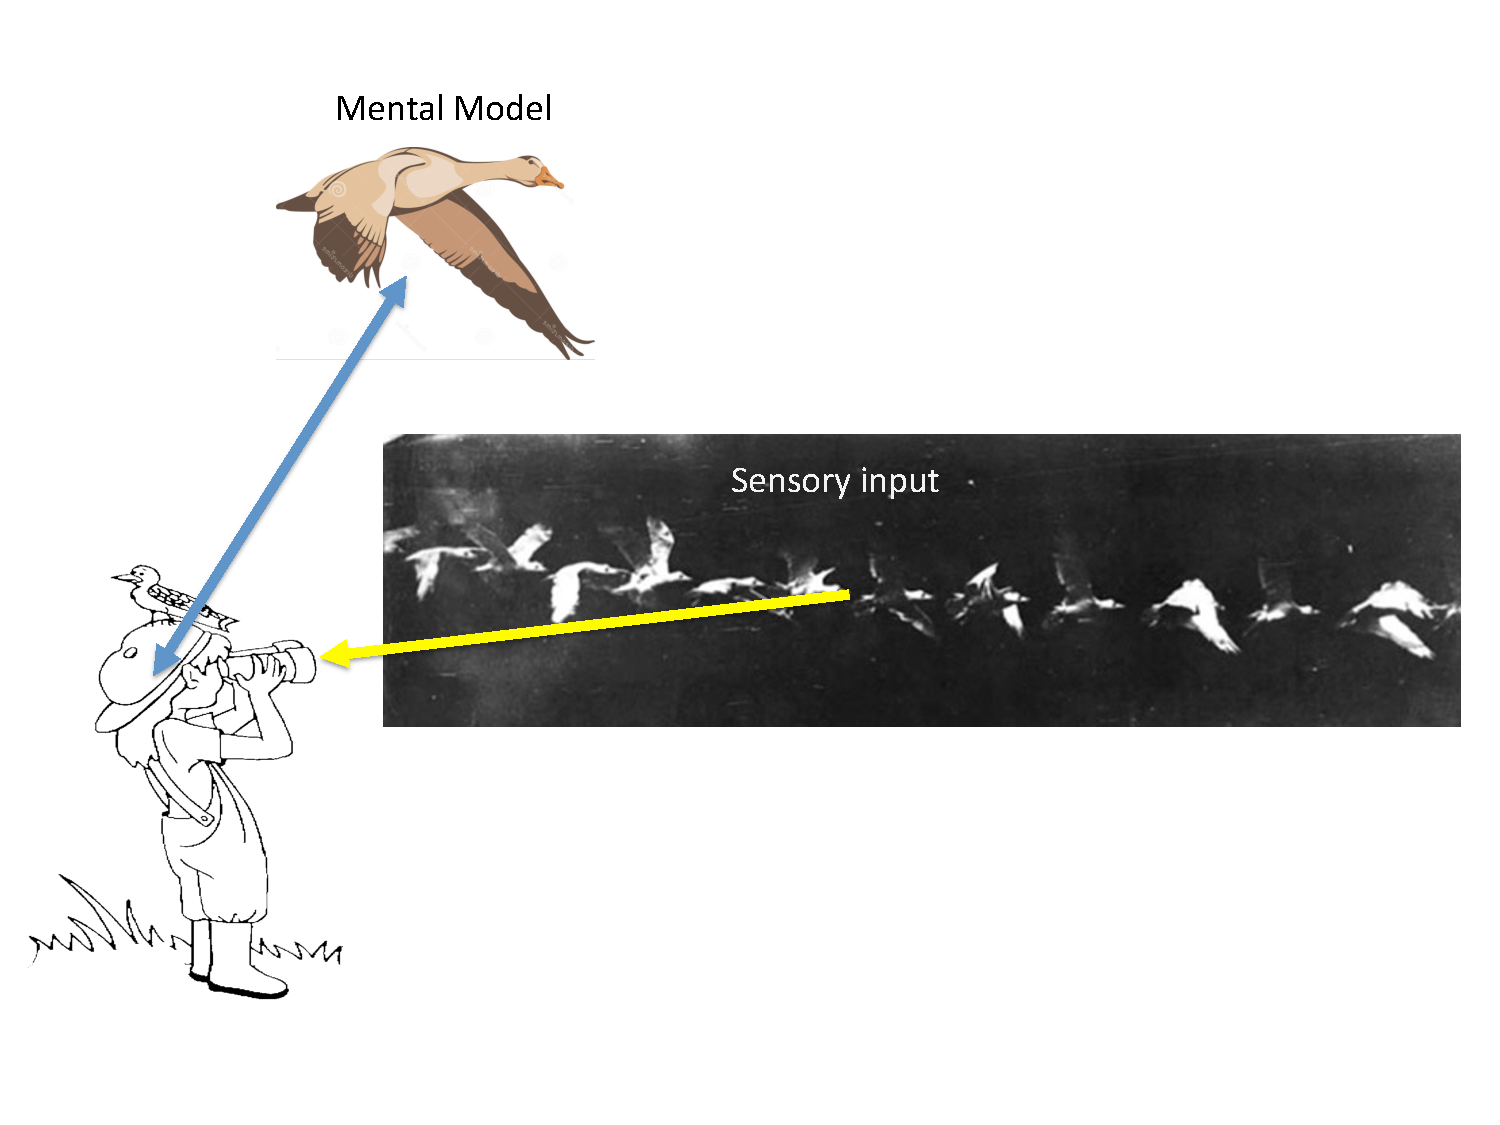
\includegraphics[width=\columnwidth]{TrackingGeese.pdf}
\caption{Bird Tracking Example}
\label{fig:trackingGeese}
\vspace{-0.4cm}
\end{figure}

\emph{The insufficieny of sensory data:} Note that the sensory
information is neither neccessary nor sufficient for tracking the
bird. It is not neccessary because objects other than the bird are
irrelevant to the task. It is not sufficient because poor focus,
glare, obstruction and other sources of {\em noise} and {\em
  distortion} might make it impossible to locate the bird in any single
frame.

\emph{Data integration using a model:} The brain transforms this
imperfect information into pan and tilt commands to the head and eyes
of the observer so as to keep the bird in the center of the field of
view. To do so the brain uses a {\em model} of the bird in flight. In
this simple example the model represents the {\em appearance} of the
bird in terms of shapes and colorsthe {\em movement} of the bird in
space. If this is an experienced bird watcher, the model is highly
detailed and specific and is {\em adapted} to the particulars of the
task.

\emph{Parameters and state:} A typical model consist of two parts:
fixed (or slowly varying) {\em parameters} and a rapidly varying {\em
  state}. In the bird tracking example the parameters might include
the appearance of the bird from different angles and at different
stages of flapping the wings. It contains also a characterization of
the range of speeds and altitudes at which the bird typically flies
and of typical changes in the flight direction.  The {\em state} in
the bird tracking example might include of the pan and tilt angles,
the change rates of these angles, the direction from which the bird is
viewed and the phase of the wing flap cycle.

\emph{Correspondance:} A model is a representation of {\em real world
  system}. If the model is good, then there is a one to one
correspondance between the parameters of the model and the
characteristics of the physical system and between the state of the
model and the state of the system. A main goal of \projName\ is to
construct models whose state corresponds to the state of the real world.

\emph{Learning, tracking and loss functions} the parameters and the
state of the model are adjusted according to the sensory data. We call
the adaptation of the parameters ``learning'' and the adjustment of
the state ``tracking''. The goal of both learning and tracking is to
minimize a {\em loss function}. The loss function takes as input
sensory data and a model and outputs a non-negative number. If the
loss (or the average loss) is low we say that the model {\em conforms}
with the data.


\emph{Models and compression} One of the ways in which a conforming
model can be used is to {\em compress} the data. Models that conform
to the data can usually be transformed into {\em predictive} models
which predict future values based on past values. Compression is
achieved by encoding the data as a sequence of differences between the
prediction and the measurements. If the predictions are accurate, the
number of bits required to store the differences is much smaller than
the number of bits required to store the raw data. Compression comes
in two flavors: {\em lossless compression} (such as the Lempel-Ziv method)
allows perfect reconstruction of the original signal, while {\em lossy
  compression} (such as DPCM, MP3 and JPEG2000) allows only
approximate reconstriction. On the other hand, the compression ratio
achieved by lossy compression is typically much higher.

\emph{Compression Bias} Lossy compression is not free. Lossy
compression using a poorly chosen model which does not represent the
measured reality can create artifacts in the reconstructed data. In
some cases the artifacts can mask important state data.

\emph{Noise reduction} If the model is well chosen and it's parameters
and state corrspond to those of the measured reality, the
reconstructed data can be a {\em better } representation of the state
of reality than the raw signal. That is related to the fact that
common types of noise, in particular {\em additive white noise} have high
information content (entropy) and are impossible to compress. Removing
the white noise component results in a win-win situation where the
compressed signal is highly comressed and the reconstructed signal is
a better representation of the state of reality than the raw signal.

\subsection{Notation}

We use the following notation to represent the above mentioned
concepts.

\newcommand{\cM}{{\cal M}}
\newcommand{\cSM}{{\cal SM}}

\begin{itemize}

\item Denote the spatiotemporal space by $X$ and call a particular
  element $x \in X$ a point. (Typically $a$ defines both location and time).

\item A measurement is a pair $(x,y)$ where $x$ is the location (in
  space and time) in which the measurement was taken and $y \in Y$ is the
  quantity measured. We will refer to $Y$ as the outcome space. The
  outcome space can be a scalar (for example, a temperature
  measurement), a vector (for example, an image) or a (potentially
  infinite) sequence of measurements:$y_1,y_2,y_3,\ldots$.

\item A stateless model $\cM$ is a is a function that maps from $X$ to a
  prediction space $\Lambda$.  

\item The outcome space $Y$ and the prediction space are linked
  through a Loss function $\gamma:\Lambda \times Y \to R^+$ where
  $R^+$ is the set of non-negative reals. A good prediction is one
  which induces a small loss. Below we describe a few popular
  outcome/prediction pairs.

\item A model with state (also called a ``filter'') which we denote by
  $\cSM$, consists of a state $s \in S$ and two
  functions $A: S \times Y \to S$ and $O: S \to \Lambda$. The
  model assumes that the time is descrete and sequential.
  The initial state $s_0$ is assumed to be of no long term importance
  (i.e. the markov model defined by the model plus nature is rapidly
  mixing). The model takes as input a sequence of inputs
  $y_1,y_2,\ldots$ and performs the following two steps for $t=1,2,3,\ldots$:
  \begin{enumerate}
    \item Update state (Track): $s_t = A(s_{t-1},y_t)$
    \item Produce prediction: $\lambda_t=O(s_t)$
  \end{enumerate}

\item A learning algorithm takes as input a {\em training set}, which
  is a set of $m$ measurements$\{(x_1,y_1),\ldots,(x_m,y_m)\}$ and
  outputs a model $\cM$ or $\cSM$ which  has low loss with respect to
  a given loss function $\gamma$.
\end{itemize}

\subsection{Queries}

\subsubsection{Simple Queries}

A point query specifies a location $x \in X$ and asks the model to
make a prediction on $x$, where the prediction an element in the
outcome space, i.e. $y \in Y$. Typical loss functions for this case
are $(\cM(x)-y)^2$ or $|\cM(x)-y|$.

A range query specifies a location $x$ and asks the model to predict a
range $[a,b]$ (or, more generally, a set) that contains the outcome
$y$. The loss function that is associated with this case is the binary
function that is $0$ in the range $[a,b]$ and $1$ outside of this
range.

\subsubsection{Statistical Guarantees for simple queries}

Statistical guarantees are stated about a model as a whole, not about
the prediction on specific locations. There are three major types of
guarantees:

\begin{itemize}
\item {\bf Worst-case or max-norm guarantees} These are guarantees of
  the form: with probability 1-over the random choice of the training
  set the learning algorithm generates a model $\cM$ such that: For
  any measurement $(x,y)$ the outcome y is within predicted range
  $[a(x),b(x)]=m(x)$ Note that in this case evaluating using a model
  that predicts a single number and a loss function is a special case
  of the range model.
\item{\bf Average-case guarantees} In this case the test locations are
  chosen using the same distribution as that of the training set. The
  guarantee takes the form: with probability 1-over the random choice
  of the training set the learning algorithm generates a model m such
  that: A test example (test measurement) $(x,y)$ is chosen
  independently at random according to the same distribution that
  generated the training set. Our guarantee is on the expected value
  of the loss function $E(x,y)m(x),y$ more precisely, we say that with
  probability 1-over the random choice of the training set the
  learning algorithm generates a model m such that: $E_{(x,y)}[\gamma(m(x),y)]$ In
  this case a model that predict with a range can be given an
  average-case guarantee, using the range-based loss function.

\item{\bf Statistical significance} This guarantee is the weakest, and
  therefore the easiest to prove. In this case we compare the model we
  generated with a model that was agreed upon a-priori. That
  agreed-upon model is the {\em Null Hypothesis}. The null hypothesis
  defines a distribution over the test measurements. The model
  generated by the learning algorithm is called the {\em Alternative
  Hypothesis}. The type of guarantee given in this case is that the
  probability of the training set according to the Null hypothesis is
  much smaller than the probability of the set according to the
  Alternative Hypothesis. Specifically, the P-value by which we can
  reject the null hypothesis (and adopt the alternative) is the
  probability of the training set (and any set ``more extreme than it'')
  according to the null.

\end{itemize}

\iffalse
the observation that sensor data can be stored
and processed much more efficiently if one operates not on the actual
measurements but on a model of the underlying reality that can be
built from the former. But what is a model? In statistics a model is a
statement about reality. This statement could be of any form. For
instance, a model could be a fundamental law (e.g., Newton's law of
acceleration, stating that the force vector $\vec{F}$ can be inferred
from the acceleration vector $\vec{a}$ and the mass $m$ through the
formula $\vec{F}=m \vec{a}$) or a statement about a physical quantity
in space and/or time in the past (e.g., the temperature at the
entrance of the compute science department at UC San Diego on August
19, 2014 at 9am was between 68 and 70 degrees). But it could also be a
predictive claim about the future (e.g., the average temperature of
the earth will increase by at least 5 degrees between 2014 and 2050),
or a theory (e.g., a medical theory stating that the statins decrease
the chance of a heart attack by more than 20\%).
\fi

\subsection{Model queries}
Higher order queries regard the models, rather than the raw
data. There can be queries regarding the state of the model (what are
the pan/tilt angles that would point towards the bird) or about the
parameters of the model (How does this type of bird look when seen
from a particular angle?).

To be continued.

\section{Older ``Models'' section} 

\projName\ is based on the observation that sensor data can be stored and processed much more efficiently by operating not on the actual measurements but instead on a model of the underlying reality that can be inferred from the measurements. What is a model? In statistics a model is a statement about reality, which could be in general of any form. For instance, a model could be a fundamental law (e.g., Newton's law of acceleration, stating that the force vector $\vec{F}$ can be inferred from the acceleration vector $\vec{a}$ and the mass $m$ through the formula $\vec{F}=m \vec{a}$) or a statement about a physical quantity in space and/or time in the past (e.g., the temperature at the entrance of the computer science department at UC San Diego on August 19, 2014 at 9am was between 68 and 70 degrees). But it could also be a predictive claim about the future (e.g., the average temperature of the earth will increase by at least 5 degrees between 2014 and 2050), or a  theory (e.g., a medical theory stating that the statins decrease the chance of a heart attack by more than 20\%).

Since we are interested in the processing of sensor data with a spatiotemporal component, in this work we restrict our focus to \emph{quantitative spatiotemporal models}; i.e., models that provide the value of a physical quantity for points in space and/or time. An example of a quantitative spatiotemporal model is a function outputting the temperature at the entrance of the computer science department at different points in time. Signal processing has long recognized the value of operating on models inferred from the measurements, instead of operating on the actual measurements themselves.\\

{\bf Advantages of models.} The reasons for preferring models over the raw measurements are multifold: Compared to raw sensor readings, models offer several advantages:
\iffalse
\begin{itemize}
\item \emph{They are functions with possibly infinite domains.} Raw sensor readings are merely discrete samples of an underlying continuous phenomenon (i.e., they provide values of the measured quantity only for a finite number of points in space and/or time). In contrast, models provide also all intermediate values, intuitively ``filling in" the gaps left by the raw measurements in the spatiotemporal dimensions. Having the values of the measured quantity for all points in space and/or time is especially important when joining two spatiotemporal signals on their spatiotemporal component, as otherwise the two signals may not be aligned. For instance, consider the following two datasets: A dataset containing air quality measurements taken at various locations and times at UC San Diego and another dataset containing GPS readings representing the location of a person walking around campus. If we want to compute the quality of the air the particular person was breathing during the walk, we would have to join these two datasets. However a conventional relational join on the space/time attributes of the two datasets will most probably yield the empty result, as the person may have never been at the exact time and location the air quality measurements were taken. Abstracting out each of these two sets of measurements through a corresponding model solves this problem and facilitates the join, as each model will provide the values for every point in space and time.
\item \emph{They offer predictive abilities.} In addition to providing values for points in space and/or time between those for which there exist raw measurements, models may also provide predictions for future points in time, thus allowing users to ask predictive queries. For instance, an air quality model may support queries about the expected air quality tomorrow. Intuitively, the predictive nature of the models stems from the fact that instead of focusing on the actual measurements, models instead capture the (typically recurring) pattern of the underlying phenomenon.
\item \emph{They improve accuracy.} By capturing the pattern of the underlying phenomenon, models may also be able to separate the noise (inevitably introduced in raw measurements due to the limited accuracy of sensors and other random factors) from the actual signal, leading to values that are more representative of the actual reality than the sensor measurements themselves. We will discuss in Section \ref{sec:compression} how models may separate the noise from the signal returning values that are more accurate than the original raw measurements.
\item \emph{They capture uncertainty information.} Even if a model cannot completely separate the noise from the signal, it can explicitly capture the uncertainty that exists in the reported value for the measured quantity. This uncertain information is then leveraged by the query processing algorithms to generate query answers that themselves capture uncertainty. We will outline in Section \ref{sec:probabilistic-models} different ways in which a model can capture uncertainty and describe their relationship to existing works in uncertain and probabilistic databases.
\item \emph{They can be represented compactly.} Finally, models can be most of the time represented more compactly than raw measurements. This not only reduces the storage requirements for the - typically large - sensor datasets, but leads in many cases also to more efficient query execution, as queries can often be evaluated directly on the compressed model representation, as we will discuss in Section \ref{sec:query-processing}.
\end{itemize}

We next describe how \projName\ incorporates models and their associated advantages into a relational DBMS.

\fi
